\subsection{Bohr's Model}

Bohr tried to come at this from an angle that resolved the spectral line issue with Rutherford's model.
Bohr proposed that electrons move in fixed orbits, thus explaining the discrete lines of the hydrogen spectra and that atoms emit light when an electron jumps from a higher energy level to a lower one.

\begin{figure}[H]
  % https://en.wikipedia.org/wiki/Bohr_model#/media/File:Bohr_atom_model.svg 
  \centering
  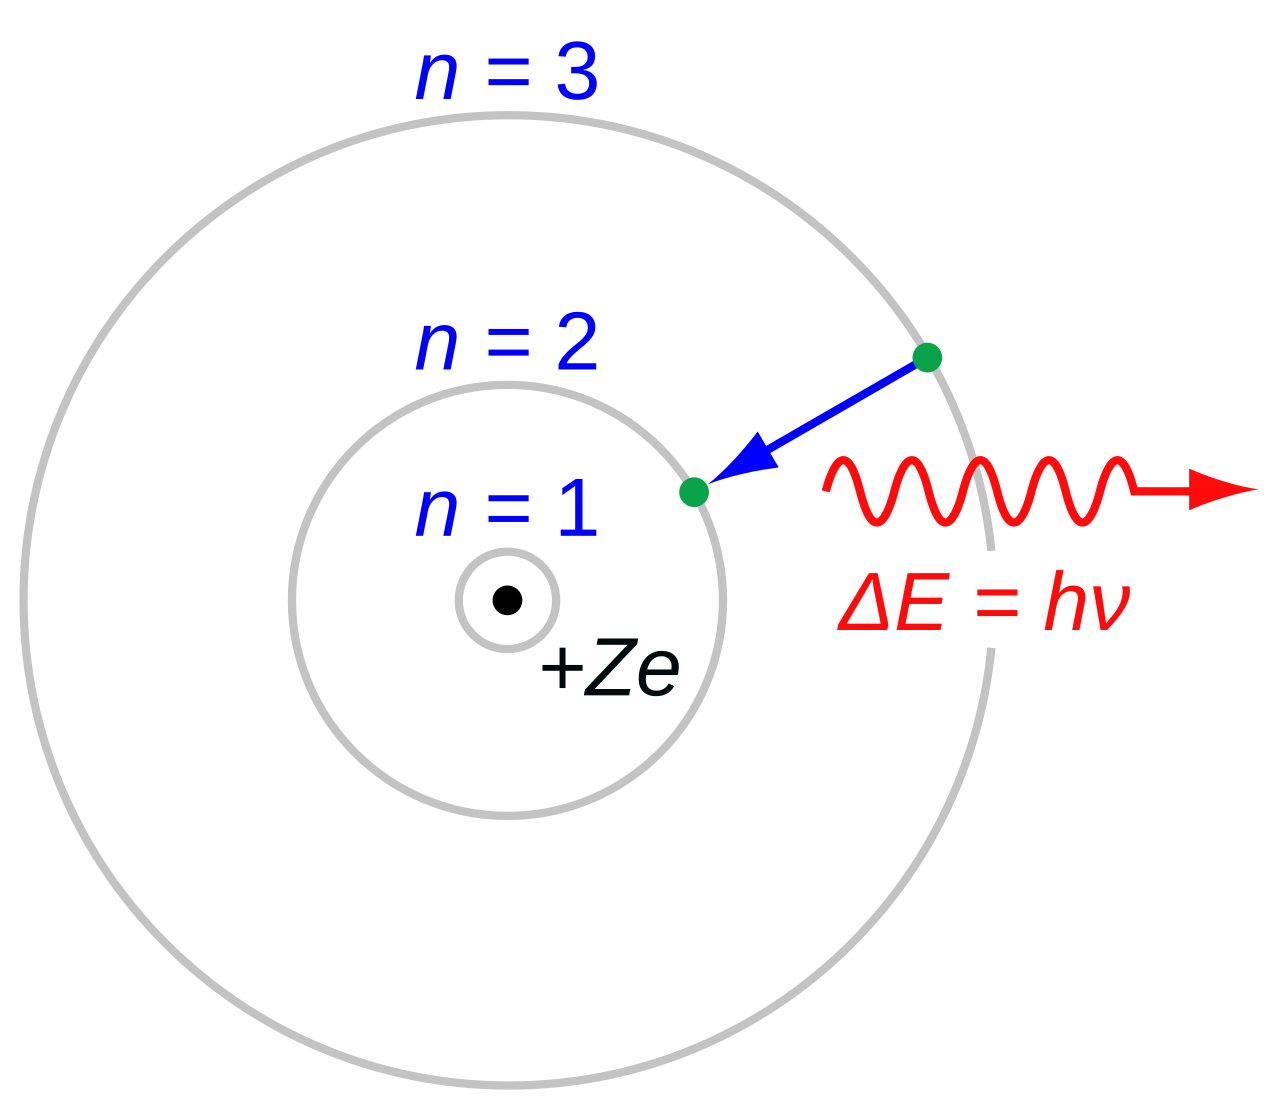
\includegraphics[width=100mm]{figures/bohr.png}
  \caption{Bohr's model of the hydrogen atom}
  \label{bohr}
\end{figure}

This still doesn't explain away why the electron doesn't collapse into the neucleus .
However, it does a very good job of modelling hydrogen and hydrogen-like atoms under most normal conditions.
The other issue with Bohr's model is that it fails to adress De-Broglie’s Hypothesis of the dual nature of matter..
To get there, we have to delve into the wonderful world of quantum mechanics.
